
\documentclass[runningheads]{llncs}

%\usepackage{natbib}
\usepackage{mathptmx}
\usepackage[utf8]{inputenc}
\usepackage{amsmath}
\usepackage{amsfonts}
\usepackage{amssymb}
\usepackage[dvips,dvipdfm,pdftex]{graphicx}
\usepackage{pgfplotstable}
\usepackage{pgfplots}
\pgfplotsset{compat=newest}
\usepackage{array}
\usepackage{booktabs}
\usepackage{morefloats}
\usepackage{etex}
\usepackage{listings}
\usepackage{float}
\usepackage{epstopdf}
\usepackage[section]{placeins}
\usepackage[ruled,linesnumbered,resetcount,algochapter]{algorithm2e}
\usepackage{caption}
%\captionsetup[table]{justification=raggedright, font=small, labelfont=bf, skip=5pt}

\begin{document}

\title{Open-set Web Genre Identification Using Distributional Features and Nearest Neighbors Distance Ratio}

%\author{Dimitrios Pritsos\inst{1} \and Anderson Rocha\inst{2} \and Efstathios Stamatatos\inst{1} }

%\institute{ University of the Aegean\\
%            Karlovassi, Samos \textendash{} 83200, Greece.\\
%            \email{\{dpritsos,stamatatos\}@aegean.gr} \and
%            Institute of Computing, University of Campinas (Unicamp),\\ Campinas, SP, Brazil
%}

\maketitle

\begin{abstract}
Web genre identification can boost information retrieval systems by providing rich descriptions of documents and enabling more specialized queries. The open-set scenario is more realistic for this task as web genres evolve over time and it is not feasible to define a universally agreed genre palette. In this work, we bring to bear a novel approach to web genre identification underpinned by distributional features acquired by doc2vec and a recently-proposed open-set classification algorithm --- the nearest neighbors distance ratio classifier. We present experimental results using a benchmark corpus and a strong baseline and demonstrate that the proposed approach is highly competitive, especially when emphasis is given on precision.

\keywords{Web genre identification \and Open-set classification \and Distributional features}
\end{abstract}


\section{Introduction}\label{sec:intro}
Web Genre Identification (WGI) aims at the association of web pages to labels (e.g., blog, e-shop, personal home page, etc.) corresponding to their form, communicative purpose, and style rather than their content. WGI can enhance the potential of information retrieval (IR) systems by allowing more complex and informative queries, whereby topic-related keywords and genre labels are combined to better express the information need of users and grouping search results by genre~\cite{Rosso2008,Malhotra:2017}. Moreover, WGI is specially useful to enhance performance of Natural Language Processing (NLP) methods, such as part-of-speech tagging (POS)~\cite{Nooralahzadeh2014} and text summarization ~\cite{Stewart:2009} by empowering genre-specific model development. 

In spite of WGI's immediate applications, there are certain fundamental difficulties hardening its deployment in practice. First, there is a lack of both a consensus on the exact definition of genre~\cite{crowston2011problems} and a genre palette that comprises all available genres and sub-genres~\cite{santini2011cross,mehler2010genres_on_web,mason2009n,sharoff2010web} to aim for. New web genres appear on-the-fly and existing genres evolve over time~ \cite{Boese2005}. Furthermore, it is not clear whether a whole web page should belong to a single genre or sections of the same web page can belong to different genres~\cite{jebari2015combination,madjarov2015web}. Finally, style of documents is affected by both genre-related choices and author-related choices \cite{petrenz2011stable,sharoff2010web}. 

Instead of aiming to anticipate all possible web-genres possible to appear in a practical scenario, it would be wiser to consider a proper handling of genres of interest while properly handling ``unseen'' genres. In this vein, 
WGI can be viewed as an open-set classification task to better deal with incomplete genre palettes \cite{Asheghi2015,pritsos2013open,pritsos2018open,pritsos2015clef,stubbe2007genre}. This scheme requires strong generalization in comparison to the traditional closed-set setup --- the one in which all genres of interest are known or defined a priori. One caveat, though, is that open-set classification methods tend to perform better while operating in not-so-high dimensional manifolds. However,  to date, most common and effective stylometric features in prior art, e.g., word and character n-grams, yield  high-dimensional spaces \cite{kanaris2009learning,sharoff2010web}. 

Aiming at properly bringing to bear the powerful algorithm modeling of open-set classification to the WGI setup, 
in this paper, we apply a recently-proposed open-set classification algorithm, the \textit{Nearest Neighbors Distance Ratio} (NNDR)~\cite{mendesjunior2016}, to WGI. To produce a compact representation of web pages --- more amenable to the open-set modelling --- we rely upon  \textit{Distributional Features} (DF) \cite{worsham2018genre} in this paper. Finally, we are also using an evaluation methodology that is more appropriate for the open-set classification framework with unstructured noise \cite{pritsos2018open}. 

We organize the remaining of this paper into four more sections. Sec.~\ref{sec:pre_work} presents previous work on WGI while Sec.~\ref{sec:approach} describes the proposed approach. Sec.~\ref{sec:experiments} discusses the experimental setup and obtained results. Finally, Sec.~\ref{sec:conclusions} draws the main conclusions of this study and presents some future work directions.

\section{Related Work}\label{sec:pre_work}
Most previous studies in WGI consider the case where all web pages should belong to a predefined taxonomy of genres \cite{Lim2005,santini2007automatic,kanaris2009learning,jebari2014pure_URL}. Putting this setup under the vantage point of machine learning, it is the same as assuming what is known as a closed-set problem definition. However, this naïve assumption is not appropriate for most applications related to WGI as it is not possible to construct a universal genre palette a priori nor force web pages to always fall into any of the predefined genre labels. Such web pages are considered \textit{noise} and include web documents where multiple genres co-exist~\cite{santini2011cross,levering2008using}. 

Santini~\cite{santini2011cross} defines \textit{structured noise} as the collection of web pages belonging to several genres, unknown during training. Such structured noise can be used as a negative class for training a binary classifier \cite{Vidulin2007}. However, it is highly unlikely that such a collection represents the real distribution of pages of the web at large. On the other hand, \textit{unstructured noise} is a random collection of pages \cite{santini2011cross} for which no genre labels are available. The effect of noise in WGI was first studied in \cite{shepherd2004cybergenre,kennedy2005automatic,dong2006binary,levering2008using}.

Open-set classification models for WGI were first
described in~\cite{pritsos2013open,stubbe2007genre}. However, these models were only tested in noise-free corpora \cite{pritsos2015clef}. Asheghi~\cite{Asheghi2015} showed that it is much more challenging to perform WGI
in the noisy web setup in comparison to noise-free corpora. Recently, \textit{Ensemble Methods} were shown to achieve high effectiveness in open-set WGI setups~\cite{pritsos2018open}.

Great attention historically on WGI has been given to the appropriate definition of features that are capable of capturing genre characteristics --- which includes but are not limited to character n-grams or word n-grams, part-of-speech histograms, the frequency of the most discriminative words, etc.  \cite{kanaris2009learning,kumari2014web,levering2008using,Lim2005,mason2009n,onan2018ensemble,petrenz2011stable,sharoff2010web}.  Additionally, some additional useful features might come from exploiting HTML structure and/or the hyperlink functionality of web pages \cite{abramson2012_URL,asheghi2014semi,jebari2014pure_URL,priyatam2013don_URL,zhu2011enhance}. Recently deep learning methods have also been tested in genre detection setups with promising results~\cite{worsham2018genre}. 

\section{Proposed Approach --- Open-Set Web Genre Identification}~\label{sec:approach}
\subsection{Distributional Features Learning}\label{sec:Gensim}
In this study, we rely upon a Doc2Vec projection methodology to representative provide distributional features for the WGI problem~\cite{rehurek_lrec,mikolov2013efficient,mikolov2013distributed}. In particular, we have implemented a special module inside our package, named \textit{Html2Vec} \footnote{A link to the source-code will be provided}
%(see \url{https://github.com/dpritsos/html2vec}) 
where a whole corpus can be used as input and one \textit{Bag-of-Words Paragraph Vectors} (PV-BOW) is returned per web-page of the corpus.

PV-BOW consists of a \textit{Neural Network} (NNet) comprising a \textit{softmax} multi-class classifier approximating $ \max{\frac{1}{T} \sum^{a=k}_{T-k}{\log{p(t_{a}|t_{a-k},...,t_{a+k})}}}$. PV-BOW is trained using \textit{stochastic gradient-descent} where the gradient is obtained via  \textit{back-propagation}. The objective function of the NNet is the maximized \textit{average log-probability} $p(t_{a}|t_{a-k},...,t_{a+k}) = \frac{e^{y_{t_{a}}}}{\sum_{i}{e^{y_i}}}$, given a sequence of training n-grams (word or character) $t_{1}, t_{2}, t_{3}, ..., t_{T}$.

For training the PV-BOW in this study, for each iteration, of the stochastic gradient descent, a \textit{text window} is sampled with size $w_{size}$. Then a random term (n-gram) is sampled from the text window and form a classification task given the paragraph vector. Thus $y = b + s(t_{1},t_{2},t_{3},...,t_{w_{size}})$, where $s()$ is the sequence of word-n-grams or character-n-grams of the sampled window. This model provides us with a representation of web pages of pre-defined dimensionality $DF_{dim}$.

%In our study we are training a PVBOW Distributional Feature model for the whole corpus. %The corpus initially is split to a set of paragraphs, as required from PVBOW. To be more specific the paragraphs are sentences split from all the document of the whole corpus. Then several models PVBOW feature models are trained for a variety of parameters and vector dimensions, explained in the experiments section below. After the model has been fitted then one vector for each web-document was inferred from the PVBOW. The final document vectors derived from \tetxit{Distributional Feature Model} are given to the open-set learning model explained below.

\subsection{Nearest Neighbors Distance Ratio Classifier}\label{sec:NNRD_Description}

The Nearest Neighbors Distance Ratio (NNRD) classifier is an open-set classification algorithm introduced in \cite{mendesjunior2016}, which in turn, is an extension upon the \textit{Nearest Neighbors} (NN) algorithm. NNRD calculates the distance of a new sample $s$ to its nearest neighbor $t$ and to the closest training sample $u$ belonging to a different class with respect to $t$. Then, if the ratio $d(s,t)/d(s,u)$ is higher than a threshold, the new sample is classified to the class of $s$. Otherwise, it is left unclassified. 

It is remarkable that, in contrast to other open-set classifiers, training of NNDR requires both known samples (belonging to classes known during training) and unknown examples (belonging to other/unknown classes) of interest. In more details, the \textit{Distance Ratio Threshold} (DRT) used to classify new samples is adjusted by maximizing the \textit{Normalized Accuracy} (NA)  $NA = \lambda A_{KS} + (1 - \lambda) A_{US}$, where $A_{KS}$ is the accuracy on known samples and $A_{US}$ is the accuracy on unknown samples. The parameter $\lambda$ regulates the mistakes trade-off on the known and unknown samples prediction. Since usually in training phase only known classes are available, Mendes et al. \cite{mendesjunior2016} propose an approach to repeatedly split available classes into two sets (known and ``simulated'' unknown). 

In our implementation of NNDR, we use cosine distance rather than the Euclidean distance because previous work found this type of distance more suitable for WGI \cite{pritsos2018open}.\footnote{A link to our implementation of NNDR will be provided upon acceptance of this paper.}

\section{Experiments}\label{sec:experiments}

%\subsection{Open-set Evaluation Methodology}
%In this study we are measuring the performance of a novel extension of the NN method, designed for open-set classification. In particular we are measuring the effect the marked-as-unknown (or marked-as-noise) genre class tags, to the open-set prediction process. To compensate the potentially unbalanced distribution of web pages over the genres, we are using the macro-averaged precision and recall measures \cite{mendesjunior2016}. Our modification calculates precision and recall only for the known classes (available in the training phase) while the unknown samples (belonging to classes not available during training) affect false positives and false negatives. To find parameter settings that obtain optimal evaluation performances we use two scalar measures, the \textit{Area Under the Precision-Recall Curve} (AUC) to the  standard \textit{11 Recall Levels} and $F_{1}$.

\subsection{Corpus}\label{sec:corpora}
Our experiments are based on~\textit{SANTINIS}, a benchmark corpus already used in previous work in WGI \cite{mehler2010genres_on_web,pritsos2018open,santini2007automatic}. This dataset comprises 1,400 English web-pages evenly distributed into seven genres (blog, eshop, FAQ, frontpage, listing, personal home page, search page) as well as 80 BBC web-pages evenly categorized into four additional genres (DIY mini-guide, editorial, features, short-bio). In addition, the dataset comprises a random selection of 1,000 English web-pages taken from the SPIRIT corpus \cite{joho2004spirit}. The latter can be viewed as \emph{unstructured noise} since genre labels are missing. 

\subsection{Experimental Setup}\label{sec:evaluation_measures}
To represent web-pages, we use features exclusively related to textual information, excluding any structural information, URLs, etc. The following representation schemes are examined: Character 4-grams (C4G), Word unigrams (W1G), and Word 3-grams (W3G). For each of these schemes, we use either Term-Frequency (TF) weights or DF features. The feature space for TF is defined by a vocabulary $V_{TF}$, which is extracted based on the most frequent terms of the training set --- we consider $V_{TF}=\{5k,10k,50k,100k\}$. The DF space is pre-defined in the PV-BOW model --- we consider $DF_{dim}=\{50,100,250,500,1000\}$.

In PV-BOW, the terms with very low-frequency in the training set are discarded. In this study, we examine $TF_{min}=\{3,10\}$ as cutoff frequency threshold. The text window size is selected from $W_{size}=\{3,8,20\}$. The remaining parameters of PV-BOW are set as follows: $\alpha=0.025$, $epochs=\{1, 3, 10\}$ and $decay=\{0.002, 0.02\}$.

Regarding the NNRD open-set classifier, there are two parameters, $lambda$ and DRT, and their considered values are: $\lambda =\{0.2, 0.5, 0.7\}$, $DRT\textit{=\{0.4, 0.6, 0.8, 0.9\}}$. All aforementioned parameters are adjusted based on grid-search using only the training part of the corpus.

For a proper comparison with prior art, we use two open-set WGI approaches with good previously reported results as baselines: Random Feature Subset Ensemble (RFSE) and one-class SVM (OCSVM) \cite{pritsos2013open,pritsos2018open}. All parameters of the baseline methods have been been adjusted as suggested in~\cite{pritsos2018open} (their experiments are based on the same corpus).

We follow the open-set evaluation framework with unstructured noise introduced in~\cite{pritsos2018open}. In particular, the open-set F1 score~\cite{mendesjunior2016} is calculated over the known classes (the noisy class is excluded). The reported evaluation results are obtained by performing 10-fold cross-validation and, in each fold, we include the full set of 1,000 pages of noise. This setup is comparable to previous studies~\cite{pritsos2018open}.

\section{Results}\label{sec:Experiments_Results}

We apply the baselines and NNDR in the SANTINIS corpus. In the training phase, we use only the 11 known genre classes while in test phase, we also consider an additional class (unstructured noise). Table~\ref{tbl:results} shows the performance of baselines and NNDR methods when either TF or DF representation schemes, based on C4G, W1G, or W4G features, are used. 

\begin{table}[t]
\center
\caption {Performance of baselines and NNDR on the SANTINIS coprus. All evaluation scores are macro-averaged.}
\label{tbl:results}
\begin{tabular}{ccccccc}
\hline
Model & Features & Dim. & Precision & Recall & AUC & F1 \\
\hline
RFSE & TF-C4G & 50k & 0.739 & \textbf{0.780} & 0.652 & 0.759 \\
RFSE & TF-W1G & 50k & 0.776 & 0.758 & \textbf{0.657} & \textbf{0.767} \\
RFSE & TF-W3G & 50k & 0.797 & 0.722 & 0.615 & 0.758 \\
OCSVM & TF-C4G & 5k & 0.662 & 0.367 & 0.210 & 0.472\\
OCSVM & TF-W1G & 5k & 0.332 & 0.344 & 0.150 & 0.338\\
OCSVM & TF-W3G & 10k & 0.631 & 0.654 & 0.536 & 0.643\\
NNDR & TF-C4G & 5k & 0.664 & 0.403 & 0.291 & 0.502 \\
NNDR & TF-W1G & 5k & 0.691 & 0.439 & 0.348 & 0.537 \\
NNDR & TF-W3G & 10k & 0.720 & 0.664 & 0.486 & 0.691 \\
NNDR & DF-C4G & 50 & \textbf{0.829} & 0.600 & 0.455 & 0.696 \\
NNDR & DF-W1G & 50 & 0.733 & 0.670 & 0.541 & 0.700 \\
NNDR & DF-W3G & 100 & 0.827 & 0.615 & 0.564 & 0.706 \\
\hline
\end{tabular}
\end{table}

First, we compare NNDR with TF features with baselines,  also using this kind of features. In this case, NNDR outperforms OCSVM. On the other hand, RFSE performed better than NNDR for Macro-F1 and Macro-AUC. This is consistent for any kind of features (C4G, W1G, or W3G). There is notable difference in the dimensionality of representation used by the examined approaches though. RFSE relies upon a 50k-D manifold while NNDR and OCSVM are based on much lower dimensional spaces. It has to be noted that RFSE builds an ensemble by iteratively selecting a subset of the available features (randomly). That way, it internally reduces the dimensionality for each constituent base classifier of the ensemble. On the other hand, NNDR seems to be confused when thousands of features are considered as it is based on distance calculations. 

Next, we compare NNDR models using either TF or DF features. There is a notable improvement when DFs are used in associated with the open-set NNDR classifier. The dimensionality of DF is much lower than TF and this seems to be crucial to improve the performance of NNDR. This is consistent for all three feature types (C4G, W1G, and W3G). NNDR with TF scheme is competitive only when W3G features are used. It has also to be noted that in all cases the selected value of parameter DRT is 0.8. This indicates that NNDR is a very robust algorithm.

Finally, the proposed approach using NNDR and DF outperforms OCSVM but it is outperformed by the strong baseline RFSE in both macro-AUC and macro F1. However, when precision is concerned, NNDR is much better. A closer look at  the comparison of the two methods is provided in Fig. \ref{fig:NNDR_W3G_Best_RFSE_Baseline}, where precision curves in 11-standard recall levels are depicted. The precision value at $r_j$ level is interpolated as follows: $P(r_j)=max_{r_j \leq r \leq r+{j+1}}(P(r))$.

The NNDR-DF model maintains very high precision scores for low levels of recall. The difference between NNDR-DF and RFSE at that point is clearer when W3G features are used. NNDR-TF is clearly worse than both NNDR-DF and RFSE. In addition, OCSVM is competitive in terms of precision only when W3G features are used but its performance drops abruptly in comparison to that of NNDR-DF. Note that the point where the curves end indicates the percentage of corpus that is left unclassified (assigned to unknown class). RFSE manages to recognize correctly larger part of the corpus, more than $70\%$, with respect to NNDR-DF that reaches $60\%$. 

%\begin{table}
%\center
%\begin{tabular}{|l|l|rcr|cr|cl|rrrr|}
%\hline
%MAX. & MODEL & FSS & $\sigma$T & ITER. &T.TYPE & DIMs &WS & DEC. & M\emph{P} & M\emph{R} & M\emph{AUC} & M\emph{F1} \\
%\hline
%F1/AUC & NNDR-DF & - & - & - & C4G & 50 & 8 & 0.002 & 0.829 & 0.600 & 0.455 & 0.696 \\
%F1/AUC & NNDR-DF & - & - & - & W1G & 50 & 3 & 0.02 & 0.733 & 0.670 & 0.541 & 0.700 \\
%F1/AUC & NNDR-DF & - & - & - & W3G & 100 & 3 & 0.02 & 0.827 & 0.615 & 0.564 & 0.706 \\
%F1/AUC & NNDR-TF & - & - & - & C4G & 5000 & - & - & 0.664 & 0.403 & 0.291 & 0.502 \\
%F1/AUC & NNDR-TF & - & - & - & W1G & 5000 & - & - & 0.691 & 0.439 & 0.348 & 0.537 \\
%F1/AUC & NNDR-TF & - & - & - & W3G & 10000 & - & - & 0.720 & 0.664 & 0.486 & 0.691 \\
%% AUC & NNDR-TF & - & - & - & W3G & 5000 & - & - & 0.738 & 0.604 & 0.437 & 0.664 \\
%F1 & RFSE-TF & 1000 & 0.5 & 100 & C4G & 50000 & - & - & 0.739 & 0.780 & 0.652 & 0.759 \\
%%AUC & RFSE-TF & 500 & 0.5 & 300 & C4G & 10000 & - & - & 0.686 & 0.831 & 0.722 & 0.751 \\
%F1 & RFSE-TF & 10000 & 0.5 & 1000 & W1G & 50000 & - & - & 0.776 & 0.758 & 0.657 & 0.767 \\
%%AUC & RFSE-TF & 1000 & 0.5 & 300 & W1G & 5000 & - & -  & 0.618 & 0.807 & 0.673 & 0.700 \\
%F1  & RFSE-TF & 1000 & 0.7 & 100 & W3G & 50000 & - & - & 0.797 & 0.722 & 0.488 & 0.758 \\
%AUC & RFSE-TF & 10000 & 0.5 & 100 & W3G & 100000 & - & - & 0.657 & 0.805 & 0.696 & 0.723 \\
%\hline
%\end{tabular}
%\caption {Performance of NNDR and RFSE on the SANTINIS coprus using TF and DF features. MP is the Macro Precision. MR is the Macro Recall. MAUC is the Area Under the Macro PR Curve. MF1 is the F1 score of the Macro Precision and Macro Recall. T.TYPE is the Terms Type. DIMs is the features model's dimensions. RFSE: FSS is the Features Subset Selection number. $\sigma$T is the sigma threshold. ITER is the number of iterations. DF: WS is the Windows Size of the text sentence. DEC is the decay parameter. }
%\label{tbl:NNDR_VS_RFSE}
%\vspace{-8mm}
%\end{table}

%\begin{figure}[t]
%\begin{center}
%    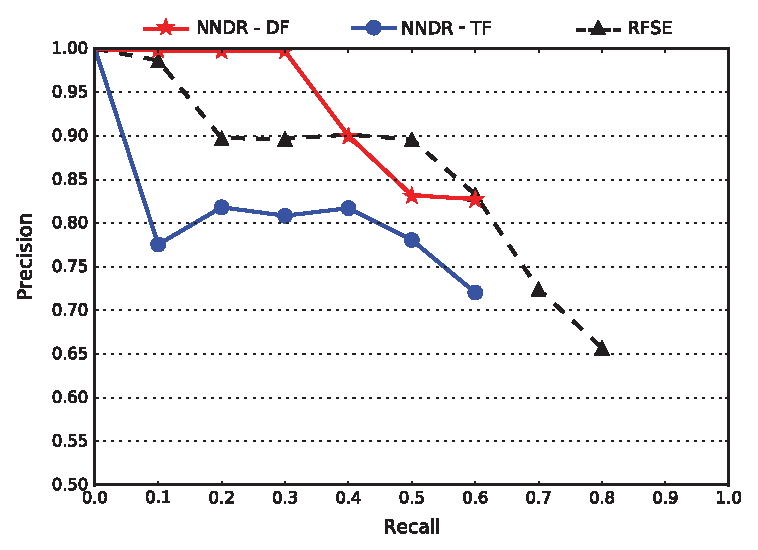
\includegraphics[scale=0.70]{NNDR_W3G_Best_RFSE-Baseline_2.eps}
%	\caption{Precision curves in 11-standard recall levels of NNDR and RFSE models.}
%	\label{fig:NNDR_W3G_Best_RFSE_Baseline}
%   \end{center}
%\vspace{-7mm}
%\end{figure}

\begin{figure}[t]
\begin{center}
    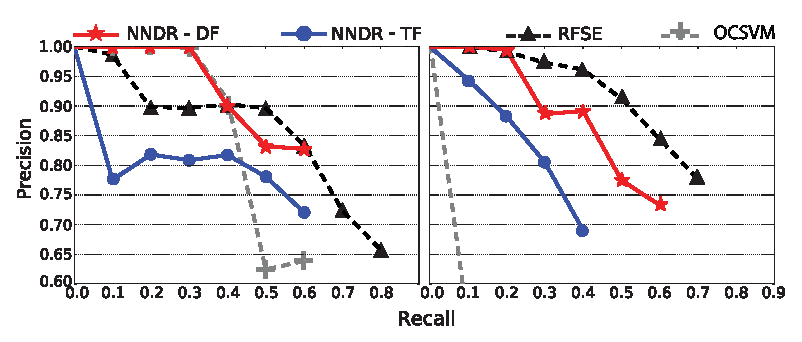
\includegraphics[scale=0.95]{NNDR_W3G-W1G_Best_RFSE-OCSVM-Baselines.eps}
	\caption{Precision curves in 11-standard recall levels of the examined open-set classifiers using either W3G features (left) or W1G features (right).}
	\label{fig:NNDR_W3G_Best_RFSE_Baseline}
	\end{center}
\vspace{-7mm}
\end{figure}



%, i.e. the remaining part after the last mark of each curve it the percentage of the corpus tha has been classified as Unknown from the algorithms.

\section{Conclusions}\label{sec:conclusions}

In this paper, we presented an experimental study focused on WGI and the use of distributional features in combination with an open-set classifier that obtained promising results in other domains. Our experiments are based on a benchmark corpus already used in prior art and a strong baseline. 

It seems that distributional features provide a significant enhancement to the NNDR open-set method. The low-dimensionality of DF is crucial to boost the performance of NNDR. Yet, RFSE proves to be a hard-to-beat baseline at the expense of relying upon a much higher representation space (usually in the thousands of features). However, with respect to precision, the proposed approach is much more conservative and it prefers to leave web-pages unclassified rather than guessing an inaccurate genre label. Depending on the application of WGI, precision can be considered much more important than recall and this is where our proposed algorithm shines. 

Further research could focus on more appropriate distance measures within NNDR specially with recent data-driven features obtained with powerful NLP convolutional and recurrent deep networks. Moreover, alternative types of distributional features could be used (e.g., topic modeling). Finally, a combination of NNDR with RFSE models could be studied as they seem to exploit complementary views of the same problem.

\bibliographystyle{splncs04}
\bibliography{ECIR2019}

\end{document}
